%%
%%  Department of Electrical, Electronic and Computer Engineering.
%%  EPR400/2 Final Report - additional results.
%%
%%  Appendix 4 describes the appendix as the place where "while the main report
%%  should contain the main results, additional results may be given here".
%%  This file therefore holds only ADDITIONAL results and the blank measurement
%%  sheets of the tests that were not carried out.  No design equation, no
%%  component value and no headline measurement was moved here: those carry the
%%  design credit and stay in Section 3 and in Section 4.
%%

\subsection{Additional results and prepared measurement sheets}
\label{sec:app-res}

This appendix holds the supporting detail of the qualification tests of Section~\ref{sec:results}: the provenance of the data sets and model checkpoints behind every quoted figure, the two measurement sheets that were prepared for the sub-tests that were never carried out, the feature definitions prescribed for the style correlation, and the distance distributions behind the overlay test.
Every figure quoted against a requirement remains in Section~\ref{sec:results}; nothing here changes a result, and the blank sheets are reproduced so that the measurement that is missing is defined rather than merely named.

\subsubsection{Provenance of the data sets and checkpoints}
\label{sec:app-prov}

Section~\ref{sec:res-qtp} states two facts that qualify every figure in it, that the harness covers ten of the thirteen writers and that the live server serves an unmeasured text checkpoint.
This sub-subsection traces both to the stored files that establish them, so that the claims can be checked rather than taken on trust.

\emph{The ten-writer subset.}
The harness was run over the eight database writers 150, 151, 152, 153, 384, 551, 552 and 588 and the two personal writers Dylan and Yeukita.
The list is set by \texttt{PERSONAL\_AUTHORS} in \texttt{qtp\_scripts/qtp\_common.py}, which names only \texttt{yeukita} and \texttt{dylan}, and the stored results confirm it: in \texttt{qtp\_data/qtp1c\_results.json} the strings \texttt{abhinav}, \texttt{owen} and \texttt{thiya} occur zero times, while \texttt{dylan} occurs 72 times and \texttt{yeukita} 96 times.
The per-writer shape-judge accuracies that make those three the weakest of the set come from \texttt{stage4\_summary.json}.
The figures that do cover all thirteen writers come from the separate verification pipeline rather than the harness: the search-judge accuracy of qualification test~1, the per-writer end-to-end run of Figure~\ref{fig:res-e2e} and the 1358-line writer identification of qualification test~2.
The 669-crop recognition figure covers the five personal writers only, which is its own data set and not the ten-writer subset.
\mustdo{re-run the qualification-test harness with \texttt{PERSONAL\_AUTHORS} set to all five personal writers, so that the style-correlation, overlay and independent-judge figures cover the same thirteen writers as the rest of the chapter.}

\emph{The checkpoints.}
The character- and word-accuracy figures of qualification test~1 were measured with two text checkpoints recorded in \texttt{qtp\_data/qtp1c\_results.json}: \texttt{meta.production\_ckpt} is \texttt{paper\_cnn\_bilstm\_ctc\_joint\_best.pt}, the checkpoint inside the best-of-$N$ search, and \texttt{meta.heldout\_ckpt} is \texttt{paper\_cnn\_bilstm\_ctc\_hf\_best.pt}, the base model used as the judge outside the search.
The recognition figures of qualification test~2 were measured with the same joint checkpoint (\texttt{verify\_text\_accuracy.py}), and the writer-identification figures with \texttt{author\_classifier\_10new\_weights.pt} for ink and \texttt{author\_shape\_10new\_weights.pt} for shape.
The deployed recogniser is a different model: \texttt{Classify.py} prefers \texttt{paper\_cnn\_bilstm\_ctc\_scratch\_best.npz} over the converted checkpoints, and that file is present, so the from-scratch checkpoint is what the server loads.
Its two writer classifiers, by contrast, are the \texttt{.npz} conversions of the \texttt{.pt} files above and agree with them on 100\% of 1358 lines to within $8\times10^{-6}$ of logit, which is why the writer figures transfer to the deployed code and the text figures do not.
\mustdo{measure character and word accuracy of the deployed \texttt{paper\_cnn\_bilstm\_ctc\_scratch\_best.npz} checkpoint on the same 669 crops, or change the server to load the joint checkpoint that was measured.}
\mustdo{record the architecture width, layer count, parameter count, optimiser, learning-rate schedule, batch size and epoch count of each named checkpoint, so that every figure in Section~\ref{sec:results} is traceable to a trained model. No hyper-parameter table or parameter count is given for any of them at present.}

\subsubsection{Per-feature and per-judge breakdown of qualification test 1}

Section~\ref{sec:res-qtp1} quotes the style correlation as one pooled number and
the two-judge comparison as one difference; both are the summary of a per-item
breakdown, which is given here because it localises the defect rather than
merely sizing it.
Figure~\ref{fig:res-features} resolves the correlation into its nine features and
Figure~\ref{fig:res-judges} the character accuracy into the two checkpoints that
read the same sixty lines, while Figure~\ref{fig:res-matched} places the
synthesis beside genuine handwriting of the identical sentences.
Table~\ref{tab:res-perfeature} lists the per-feature coefficients that
Figure~\ref{fig:res-features} plots.

\begin{figure}[h]
\centering
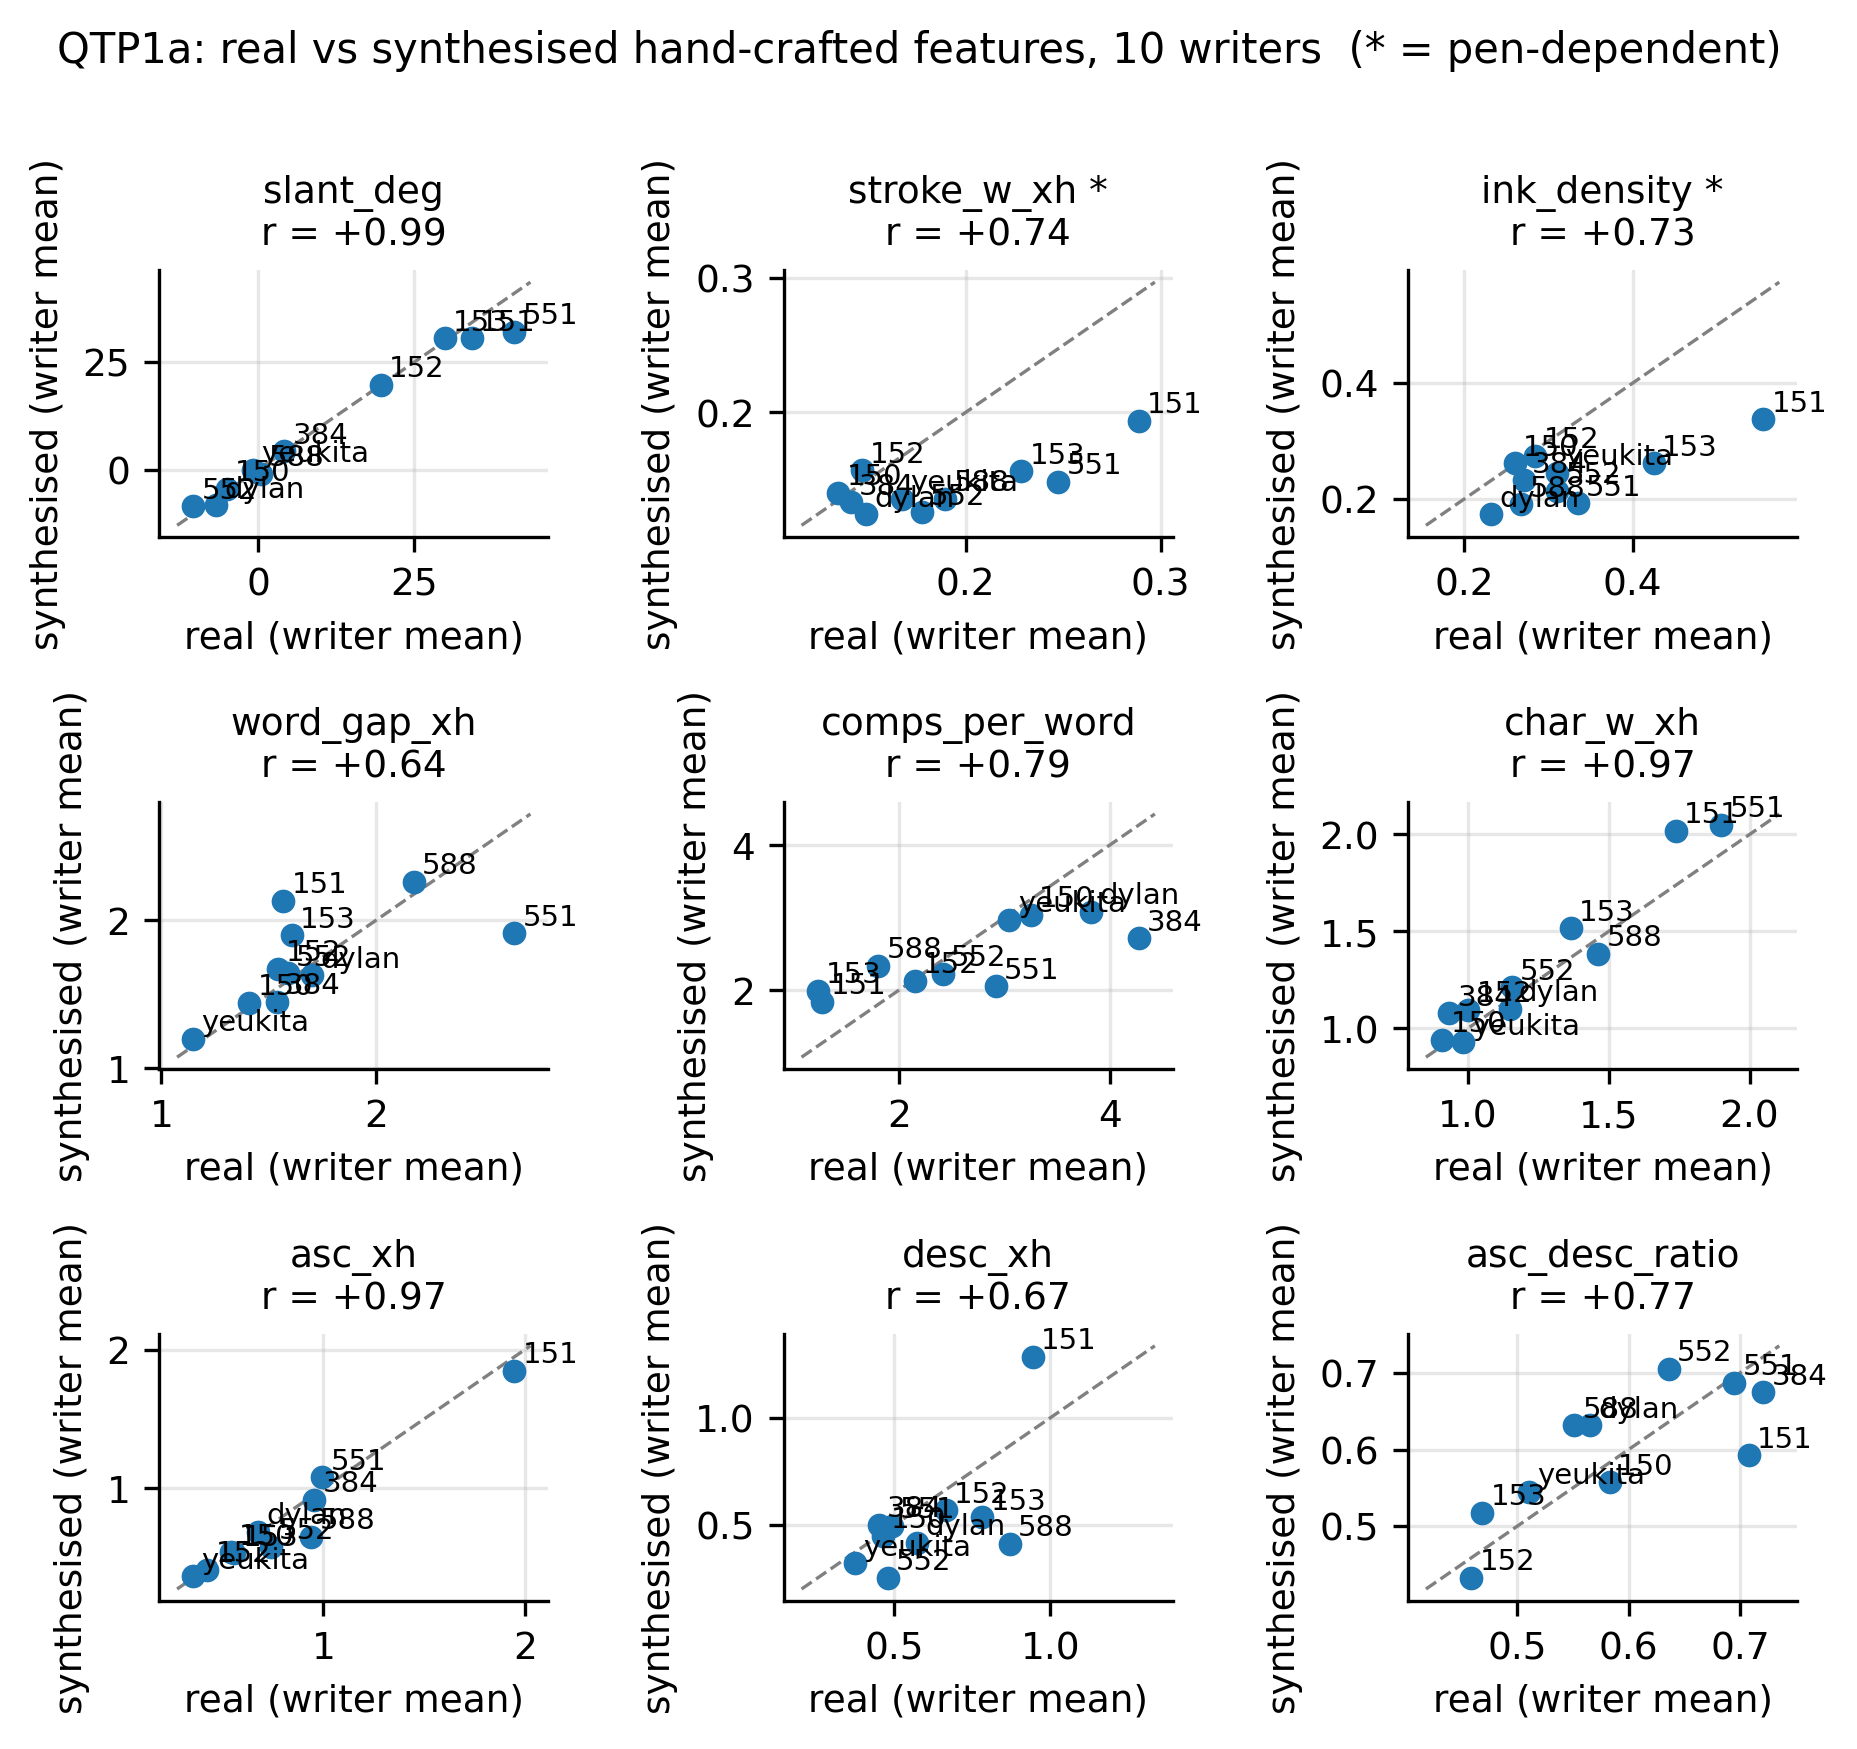
\includegraphics[width=0.99\linewidth]{Figures/qtp1_feature_scatter.png}
\caption{Style-correlation test on nine geometric features extracted by one deterministic routine from held-out real pages and from synthesised lines, for the ten writers. Each panel is one feature; the axes are the writer means. Slant, ascender and character width track the real hand closely, whereas descender and the ascender-to-descender ratio do not, which is the same defect that the word-accuracy gap identifies.}
\label{fig:res-features}
\end{figure}

\begin{figure}[h]
\centering
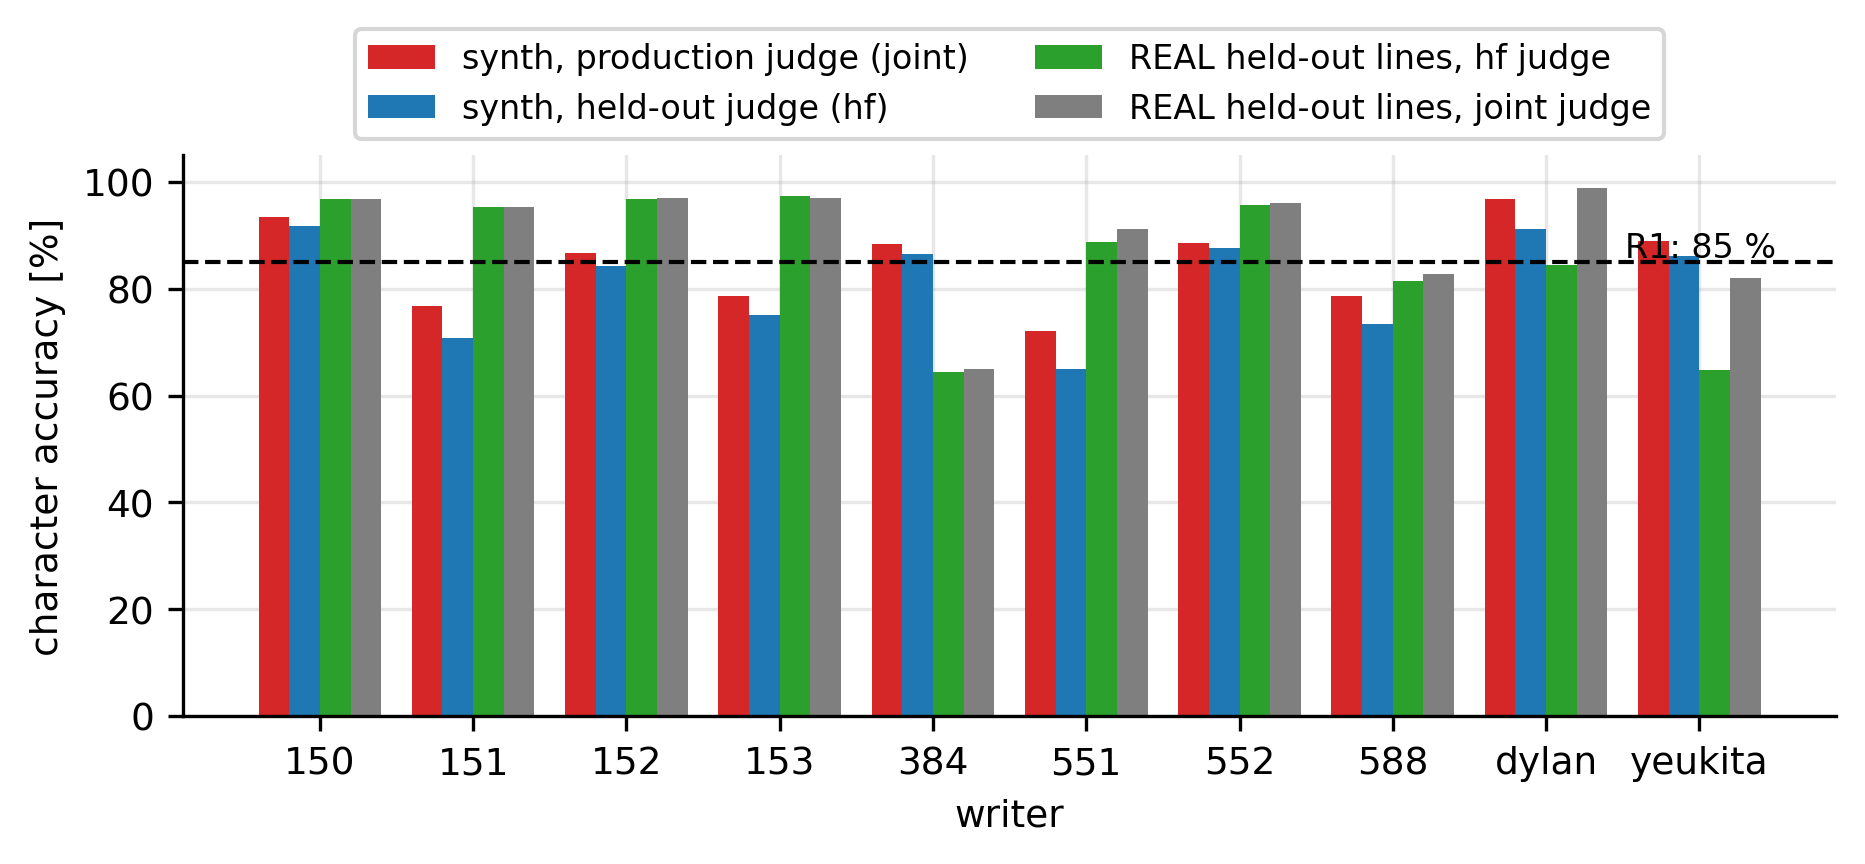
\includegraphics[width=0.85\linewidth]{Figures/qtp1_char_acc_judges.png}
\caption{Character accuracy of the synthesised text under the production recogniser and under a recogniser checkpoint that was not used to select the candidates. The independent judge scores the same output about three points lower, which quantifies how much of the apparent quality is a selection effect and simultaneously shows that the synthesis is genuinely legible rather than merely self-consistent.}
\label{fig:res-judges}
\end{figure}

\begin{figure}[h]
\centering
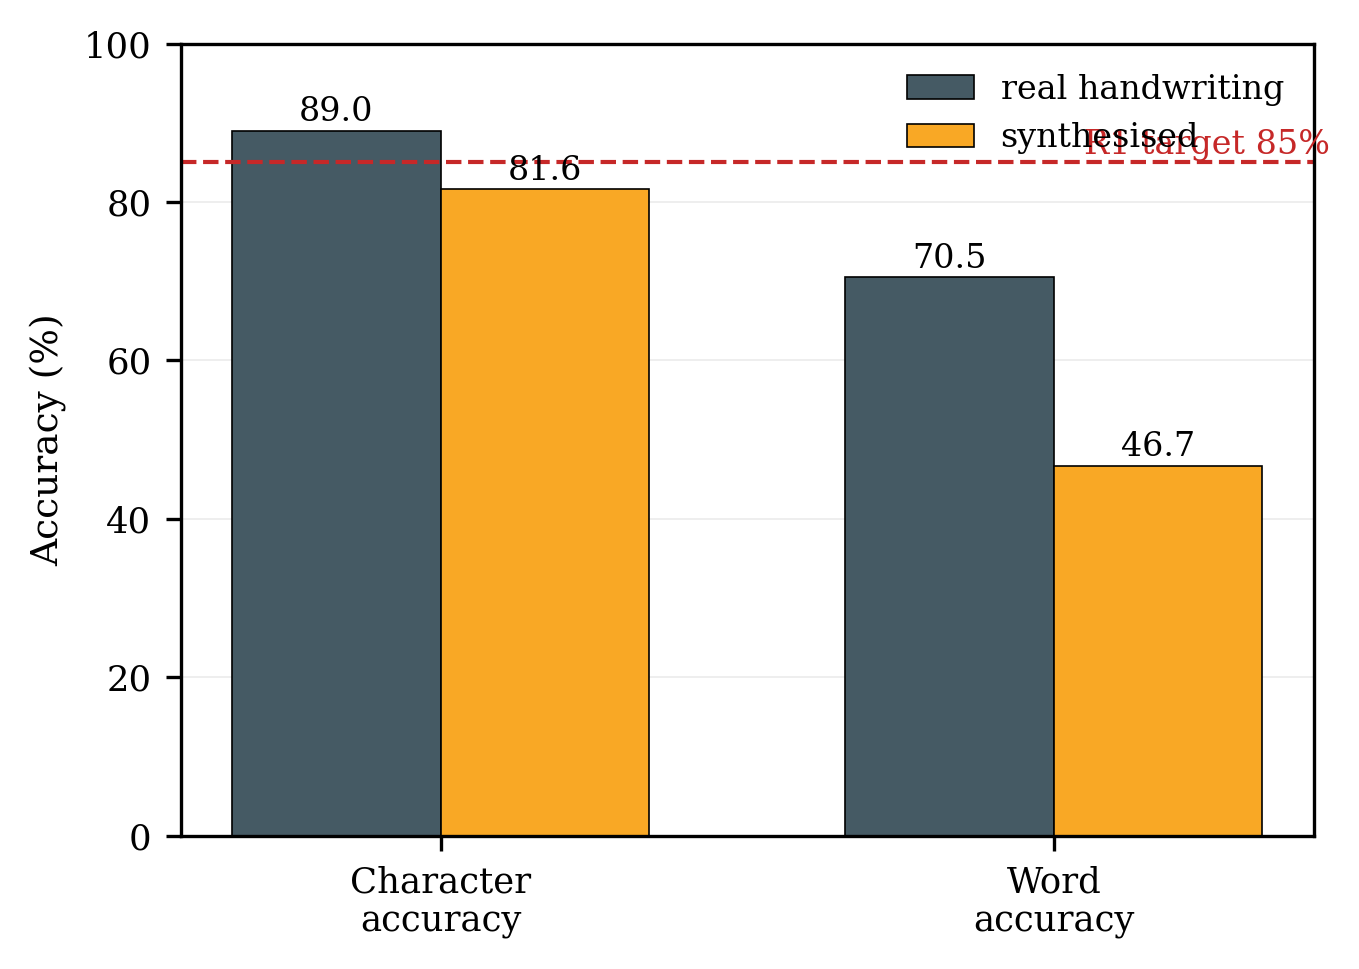
\includegraphics[width=0.85\linewidth]{Figures/res_matched_real_vs_synth.png}
\caption{Matching comparison on identical sentences: genuine handwriting of the sentence against the system's synthesis of that same sentence, both read by the same recogniser. Character accuracy is close to the target, but word accuracy divides by more than a factor of 1.5, which shows that the synthesis preserves letterforms better than it preserves word boundaries and spacing.}
\label{fig:res-matched}
\end{figure}

\begin{table}[h]
\centering
\fontsize{10}{12}\selectfont
\begin{tabularx}{\linewidth}{|>{\raggedright\arraybackslash}X|l|>{\raggedright\arraybackslash}X|l|}
\hline
\textbf{Feature} & \textbf{Pearson $r$} & \textbf{Feature} & \textbf{Pearson $r$} \\
\hline
Slant & 0.996 & Stroke width & 0.632 \\
\hline
Ascender extent & 0.974 & Word gap & 0.605 \\
\hline
Character width & 0.936 & Ascender-to-descender ratio & 0.509 \\
\hline
Components per word & 0.832 & Descender extent & 0.148 \\
\hline
Ink density & 0.680 & & \\
\hline
\end{tabularx}
\caption{Style correlation per feature across the ten harness writers, which
Figure~\ref{fig:res-features} plots and which the pooled coefficient of 0.714
reported in Table~\ref{tab:res-r1} summarises. The ordering is the result: slant
and the extent above the baseline are reproduced almost exactly, whereas the
extent below the baseline and the spacing between words are not.}
\label{tab:res-perfeature}
\end{table}


\subsubsection{Per-writer breakdowns}

The headline rates of qualification tests~1 and~2 are means over writers, and
the spread behind them is wider than the mean suggests, so the per-writer
breakdown is reproduced here in full.
Figure~\ref{fig:res-writerid} gives writer identification per writer over the
1358 real lines for both classifiers, Figure~\ref{fig:res-e2e} the end-to-end
result per writer through the G-code round trip, and
Table~\ref{tab:res-perwriter} the per-writer recognition accuracy behind the
98.61\% of qualification test~2.

\begin{figure}[h]
\centering
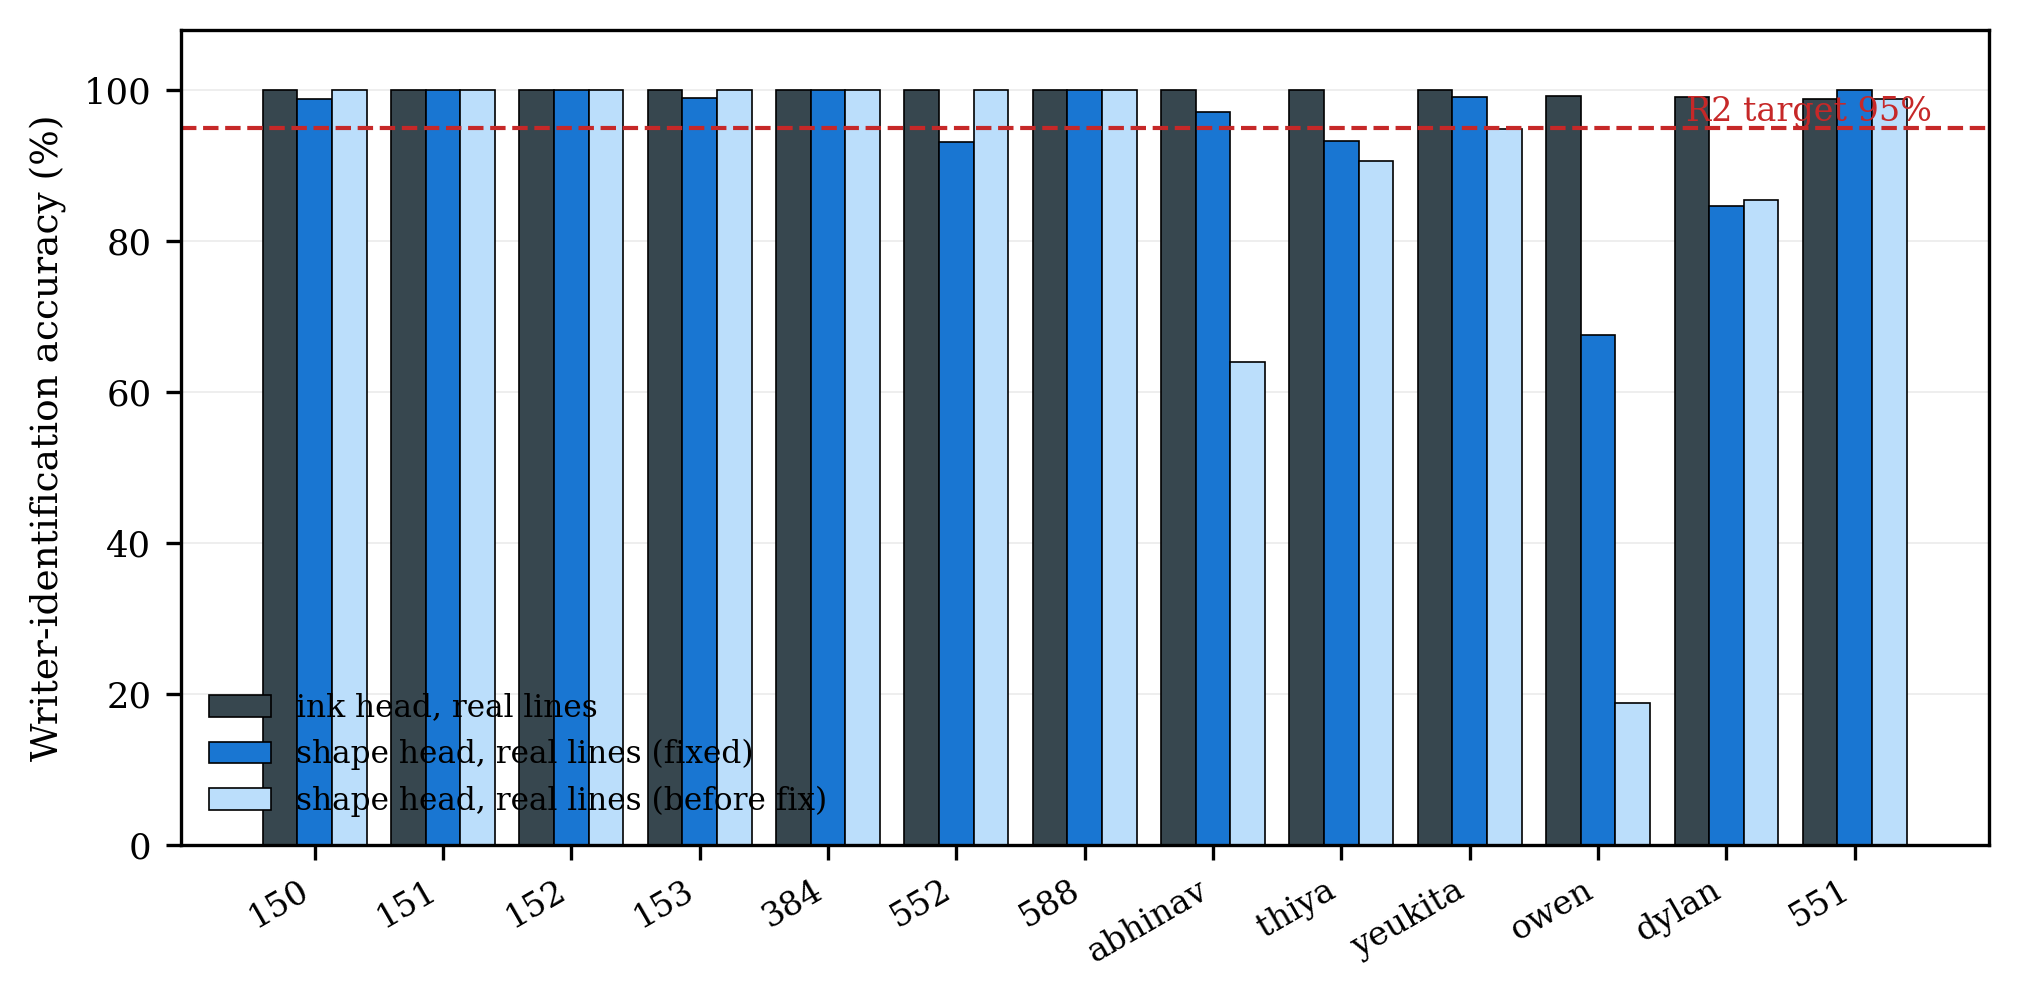
\includegraphics[width=0.85\linewidth]{Figures/res_writerid_per_author.png}
\caption{Writer-identification accuracy per writer over 1358 real lines, for the ink classifier and for the shape classifier before and after its training fault was corrected. The ink classifier is at or near 100\% for every writer. Correcting the shape classifier's training raised its overall accuracy from 83.4\% to 93.7\% and removed a systematic collapse in which 118 of Owen's 148 lines had been assigned to Yeukita. The dashed line is the 95\% target of R2.}
\label{fig:res-writerid}
\end{figure}

\begin{figure}[h]
\centering
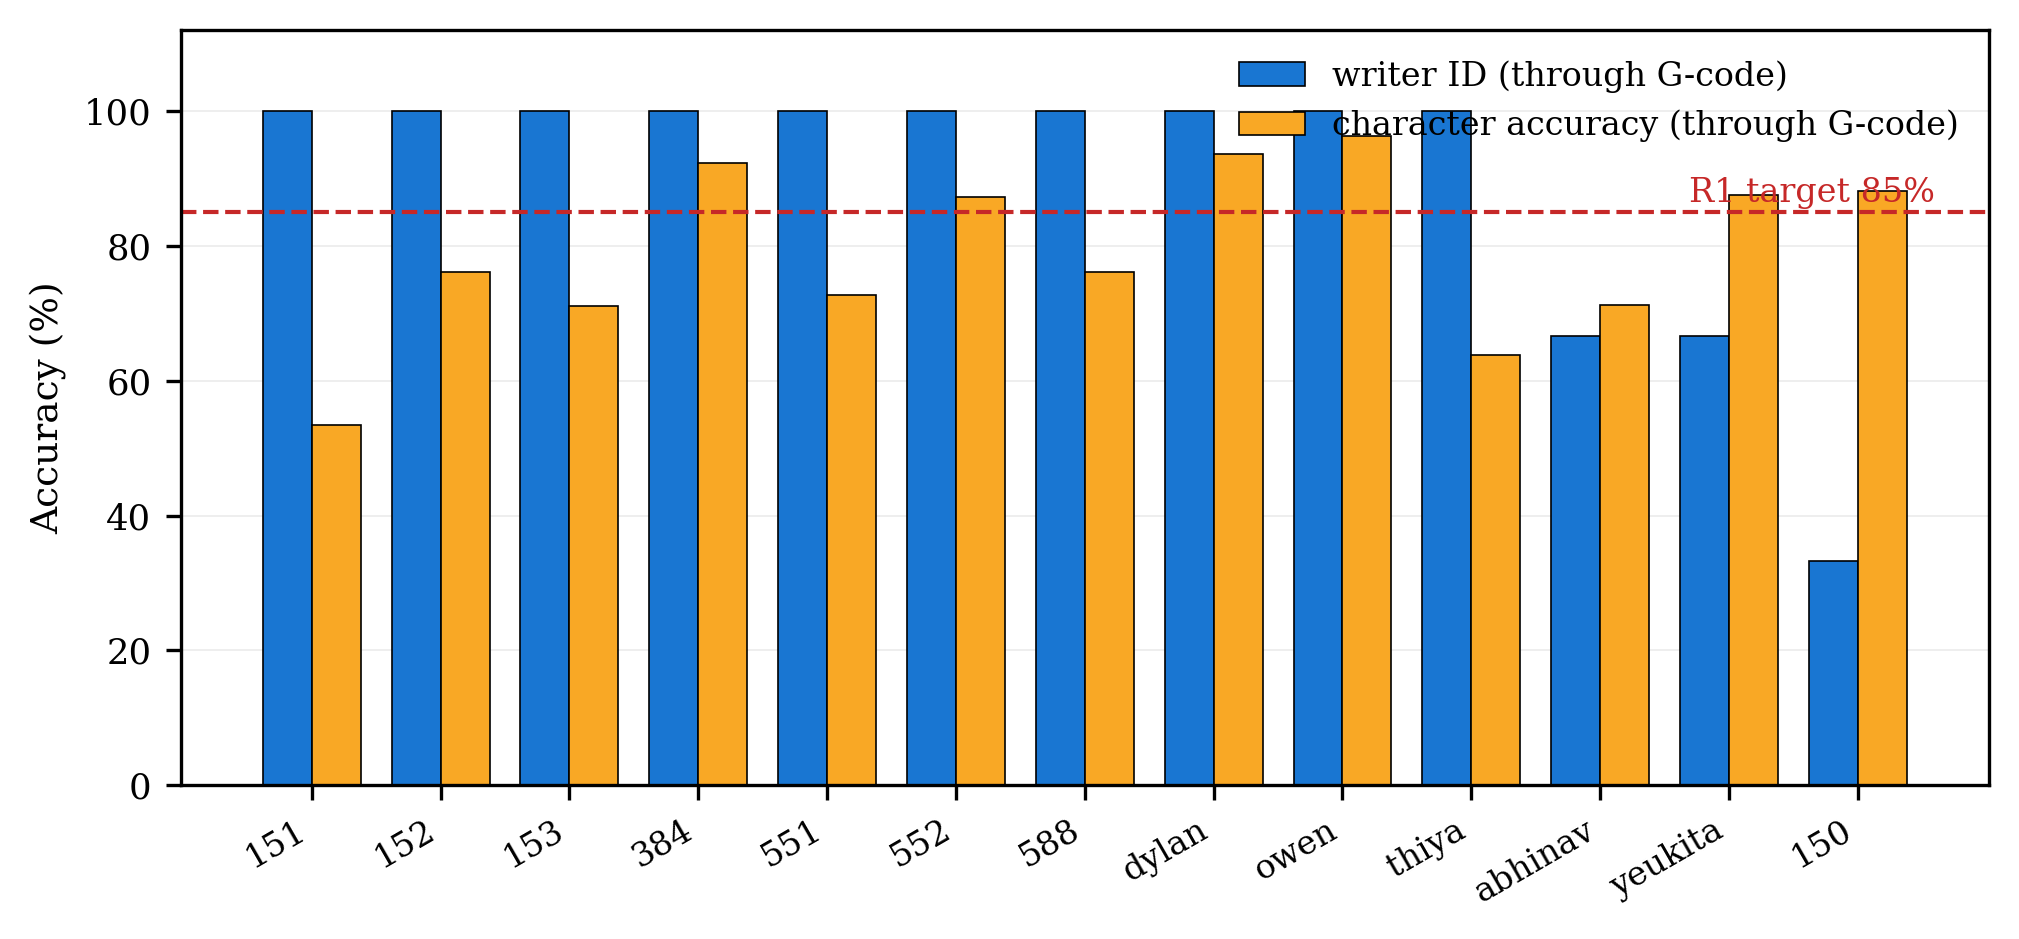
\includegraphics[width=0.85\linewidth]{Figures/res_e2e_per_author.png}
\caption{End-to-end result per writer over all thirteen writers: writer identification and character accuracy, both measured through the G-code round trip, for three novel sentences per writer at best-of-8 (\texttt{gcode\_v2\_summary.json}; shape judge \texttt{author\_shape\_10new\_weights}, text judge \texttt{paper\_cnn\_bilstm\_ctc\_joint\_best}). Ten of the thirteen writers are identified at 100\% by the shape judge; the remaining three are 150 at 33.3\% and Abhinav and Yeukita at 66.7\% each. The character-accuracy failures are concentrated in the two writers whose hands are the most joined, which is the known weak case of an exemplar synthesiser that cuts letters apart and reassembles them.}
\label{fig:res-e2e}
\end{figure}

\begin{table}[h]
\centering
\fontsize{10}{12}\selectfont
\begin{tabularx}{\linewidth}{|l|l|>{\raggedright\arraybackslash}X|}
\hline
\textbf{Writer} & \textbf{Character accuracy} & \textbf{Crops} \\
\hline
Owen & 99.15\% & 75 to 206 crops per writer; 669 in total \\
\hline
Dylan & 99.03\% & \\
\hline
Abhinav & 98.94\% & \\
\hline
Yeukita & 98.30\% & \\
\hline
Thiya & 96.46\% & \\
\hline
\end{tabularx}
\caption{Recognition accuracy per personal writer over the 669 real line crops of
qualification test 2, read by \texttt{paper\_cnn\_bilstm\_ctc\_joint\_best}. The
pooled figure is 98.61\%; Thiya, whose hand is the most joined of the five, is
the only writer more than two points below it.}
\label{tab:res-perwriter}
\end{table}


\subsubsection{Storage check of qualification test 6}

Qualification test~6 reduces to a count against a threshold, and
Figure~\ref{fig:res-storage} is the observation behind that count.

\begin{figure}[h]
\centering
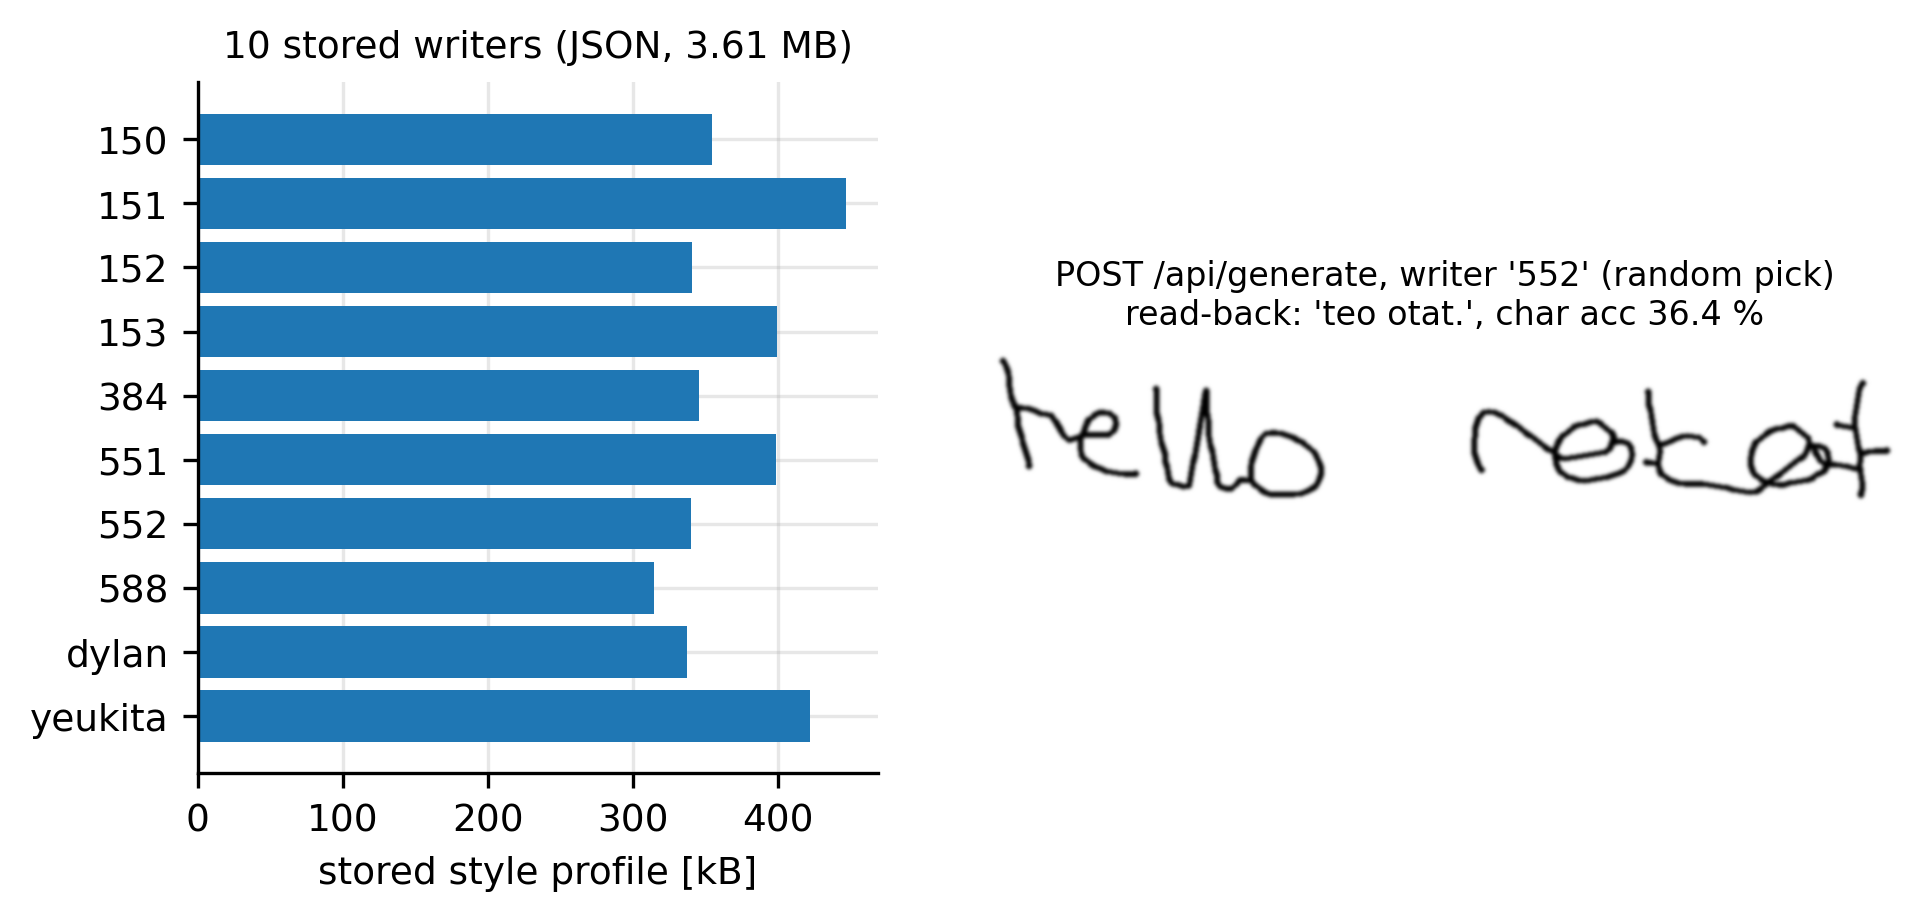
\includegraphics[width=0.85\linewidth]{Figures/qtp6_storage.png}
\caption{Storage of the writing styles. Each writer is held as a style profile and the server lists all thirteen through its author-list endpoint, against the ten required by R6.}
\label{fig:res-storage}
\end{figure}

\subsubsection{Prepared sheets for the sub-tests not carried out}

Two sub-tests were specified in full and never executed, sub-test~(d) of qualification test~1 (the blind human panel) and qualification test~5 (absolute positional error).
Table~\ref{tab:res-panel} is the worksheet printed for the panel and Table~\ref{tab:res-sheet} the data sheet printed for the positional measurements.
Both are shown exactly as printed, that is to say blank, because no rater was convened and no cross was ever drawn.

\begin{table}[h]
\centering
\fontsize{10}{12}\selectfont
\begin{tabularx}{\linewidth}{|l|X|l|l|}
\hline
\textbf{Line no.} & \textbf{Transcription written by the rater (without hint of the content)} & \textbf{Illegible characters (positions)} & \textbf{Confidence (1--5)} \\
\hline
1 & & & \\
\hline
2 & & & \\
\hline
$\vdots$ & & & \\
\hline
40 & & & \\
\hline
\end{tabularx}
\caption{Worksheet prepared for the blind human panel of qualification test 1: 30 synthesised lines and 10 genuine control lines in random order. The panel was never convened, so no worksheet was completed and the table is shown blank as it was printed.}
\label{tab:res-panel}
\end{table}

\begin{table}[h]
\centering
\fontsize{10}{12}\selectfont
\begin{tabularx}{\linewidth}{|l|l|l|l|l|l|X|}
\hline
\textbf{Repeat} & \textbf{Cross} & \textbf{$x^{\mathrm{cmd}}$ (mm)} & \textbf{$y^{\mathrm{cmd}}$ (mm)} & \textbf{$x$ meas. (mm)} & \textbf{$y$ meas. (mm)} & \textbf{$e_i$ (mm)} \\
\hline
1 & 1 & & & & & \\
\hline
1 & 2 & & & & & \\
\hline
$\vdots$ & & & & & & \\
\hline
\end{tabularx}
\caption{Data sheet prepared for the absolute positional error of qualification test 5; one row per cross and repetition, together with the scanner scale check and the registration check. No row was ever completed, because the test was not carried out.}
\label{tab:res-sheet}
\end{table}

\subsubsection{Features prescribed for the style correlation}

The style-correlation sub-test of qualification test~1 compares geometric features extracted by one deterministic routine from held-out real pages and from synthesised lines.
Table~\ref{tab:res-features} defines the features as they were prescribed in the protocol; the extractor that produced the measured correlation implements this set extended to the nine features reported in Table~\ref{tab:res-r1}.
The definitions are given here rather than in Section~\ref{sec:results} because they fix the measurement rather than report a result.

\begin{table}[h]
\centering
\fontsize{10}{12}\selectfont
\begin{tabularx}{\linewidth}{|>{\raggedright\arraybackslash}p{3.3cm}|X|}
\hline
\textbf{Feature} & \textbf{Definition} \\
\hline
Slant & Shear angle (degrees) that maximises the variance of the column ink projection of the line. \\
\hline
Stroke width & Median stroke width from the distance transform at the skeleton, divided by $x_{\mathrm{h}}$. \\
\hline
Ink density & Fraction of ink pixels inside the core band between the baseline and the x-height line. \\
\hline
Word gap & Median horizontal gap between words (gaps larger than $0.5\,x_{\mathrm{h}}$) divided by $x_{\mathrm{h}}$. \\
\hline
Connectedness & Number of connected ink components divided by the number of characters of the text. \\
\hline
Character width & Line width divided by the number of characters, divided by $x_{\mathrm{h}}$. \\
\hline
Ascender/descender ratio & (Height of the ascender zone plus depth of the descender zone) divided by $x_{\mathrm{h}}$. \\
\hline
\end{tabularx}
\caption{Hand-crafted style features prescribed for the correlation and retrieval of qualification test 1. The extractor that produced the measured correlation implements this set extended to the nine features listed in Table~\ref{tab:res-r1}.}
\label{tab:res-features}
\end{table}

\subsubsection{Distance distributions behind the overlay test}

The overlay test of qualification test~1 reduces to two numbers in Table~\ref{tab:res-r1}, the ratio of matched to mismatched distance and the area under the curve.
Figure~\ref{fig:res-dist} gives the distributions those two numbers summarise, which show how far the two populations actually overlap.

\begin{figure}[h]
\centering
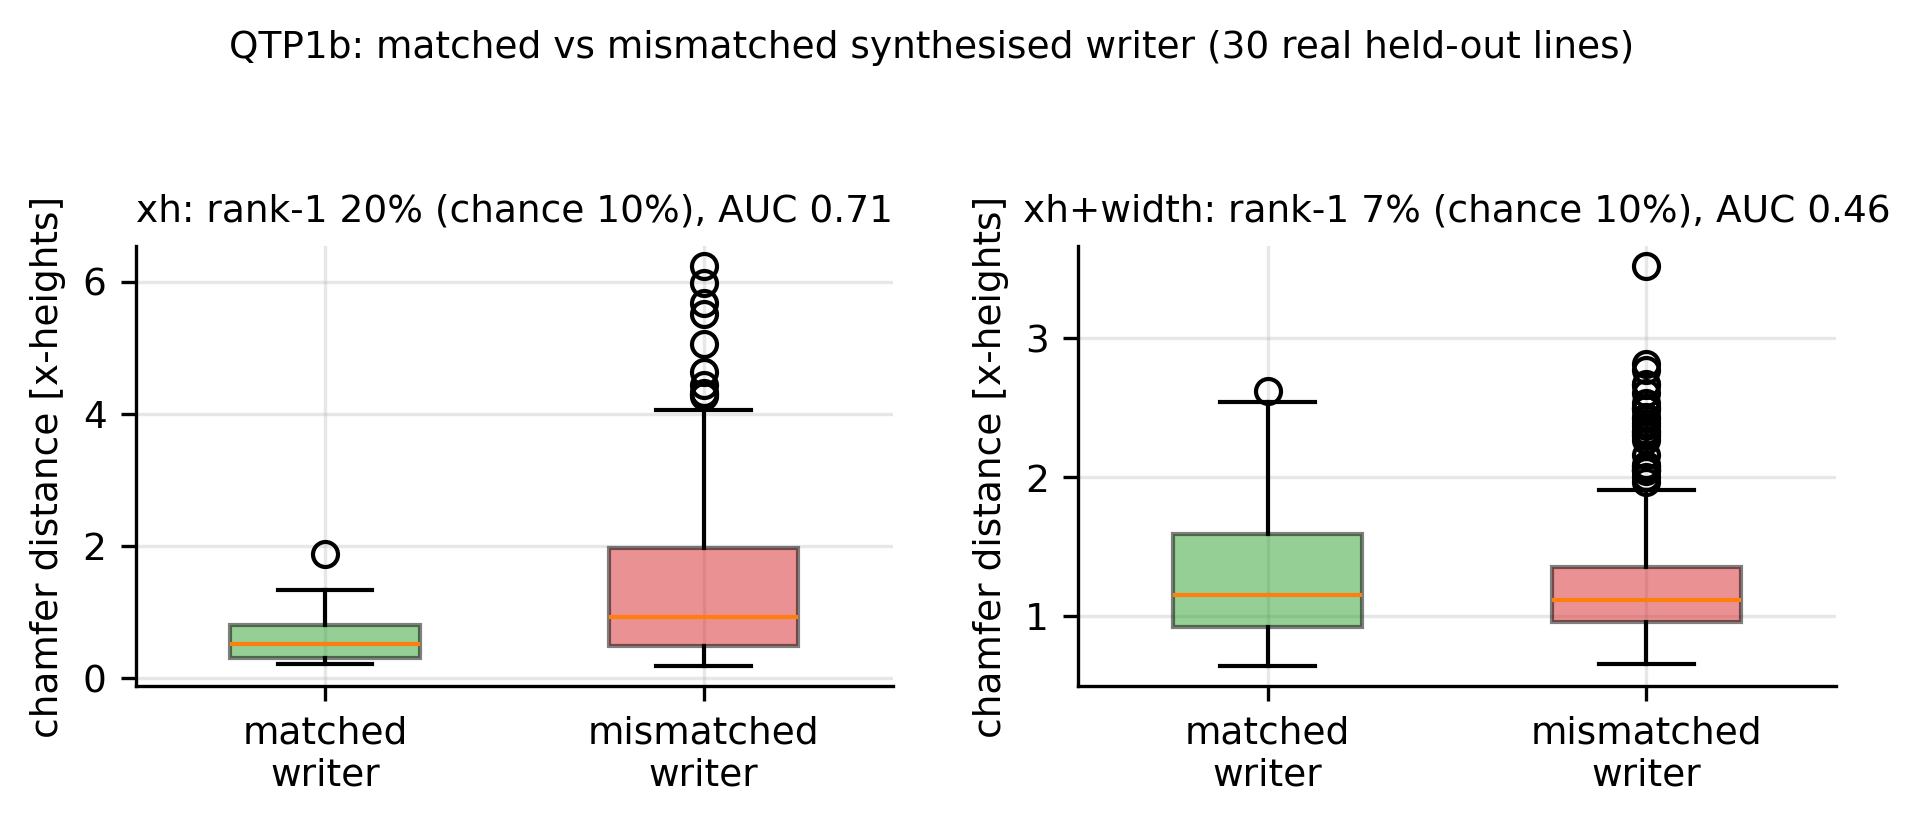
\includegraphics[width=0.93\linewidth]{Figures/qtp1_matched_vs_mismatched.png}
\caption{Distributions of the matched and mismatched overlay distances. The two distributions overlap but their means are separated by a factor of about 2.2 on the chamfer measure, giving an AUC of 0.71: the synthesis carries real writer information, but it is far from indistinguishable from the hand it imitates.}
\label{fig:res-dist}
\end{figure}
